\subsection{Classifying plant sounds}
\subsubsection{Convolutional Neural Networks (CNN's)}
Convolutional Neural Networks (CNNs) form the base for deep learning in computer vision and, as such, the field of machine learning. CNNs can process grid-like data, and no technique can process images better than CNNs. They have shown efficiency in dealing with imagery that is visual because they make use of a model in a very hierarchical manner, which processes the data in consecutive layers of processing. These networks use convolutional layers, pooling layers, and fully connected layers in the feature extraction process thus making them highly effective for tasks such as image and sound classification.\cite{oshea_introduction_2015}

This type of architecture learns automatic and adaptive spatial hierarchies of features from the input. The convolutional layer applies some learnable filters on the input in order to extract spatial features like edges and textures. Every filter is small spatially but runs through the full depth of the input volume. This way, the network is able to detect features at different locations in the input. The pooling (or subsampling) layer then reduces the spatial size of the representation by down-sampling, and that aids in controlling the overfitting problem because the number of parameters and calculations in the network is reduced. \cite{oshea_introduction_2015}

CNNs have been proven to be very good for tasks related to sound classification owing to their excellent exploitation of the invariance property of the input. This is because the fact that CNNs are capable of learning and picking up the spectro-temporal patterns present in the data that distinguish different types of sounds. When applied to sound data, which is commonly in a spectrogram representation, this can be manifested by being able to identify different patterns related to a difference in sound or soundscape. \cite{salamon_deep_2017, piczak_environmental_2015}

Some of the studies have shown the potential of CNNs in sound classification and therefore indicate the possible breakthrough in detection and classification of environmental sounds from different datasets. Such sounds include urban noise, natural soundscapes, and man-made, among others. It clearly states that the performance of CNNs can be significantly enhanced in sound classification tasks by applying techniques like data augmentation that artificially enhances the diversity of the training set through time stretching, pitch shifting, and adding background noise transformations. These regularization approaches have been shown to improve the robustness of the model, hence also translating into better generalization capability and better performance on unseen data. \cite{salamon_deep_2017, piczak_environmental_2015}

Convolutional Neural Networks were used for classifying the sounds emitted by stressed plants, such as greenhouse noises and drought-stressed tomato sounds. The Python 3.6 programming language was used to build these models using Keras library with the tensorflow backend. In its design, there are three blocks where each of them contains two 1D convolution layers with ‘relu’ activation followed by a max pooling layer and a dropout layer which ended up with a fully connected layer with ‘relu’ activation and another dropout layer. The final layer for binary classification has sigmoid activation function meanwhile for multi-class classification (three categories), softmax activation is used. \cite{Cell_Sounds_emitted_by_plants}

\subsubsection{Support Vector Machines (SVM's)}
Support vector machines (SVMs) are a supervised learning method that can be used for classification, regression, and outliers detection. They have been most popularly used to classify two-group data sets. The classifier is developed by Vapnik in the 1990s based on the concept of decision planes that define decision boundaries. A decision plane is one that separates between a set of objects having different class memberships.

The SVM works by finding the hyperplane which best divides a dataset into two classes. Support vectors are the data points nearest to the hyperplane. The distance between the hyperplane and these support vectors constitutes as margin. The further apart these support vectors are from each other, and from the margin, the more accurate your classifier will be.

\begin{figure}
    \centering
    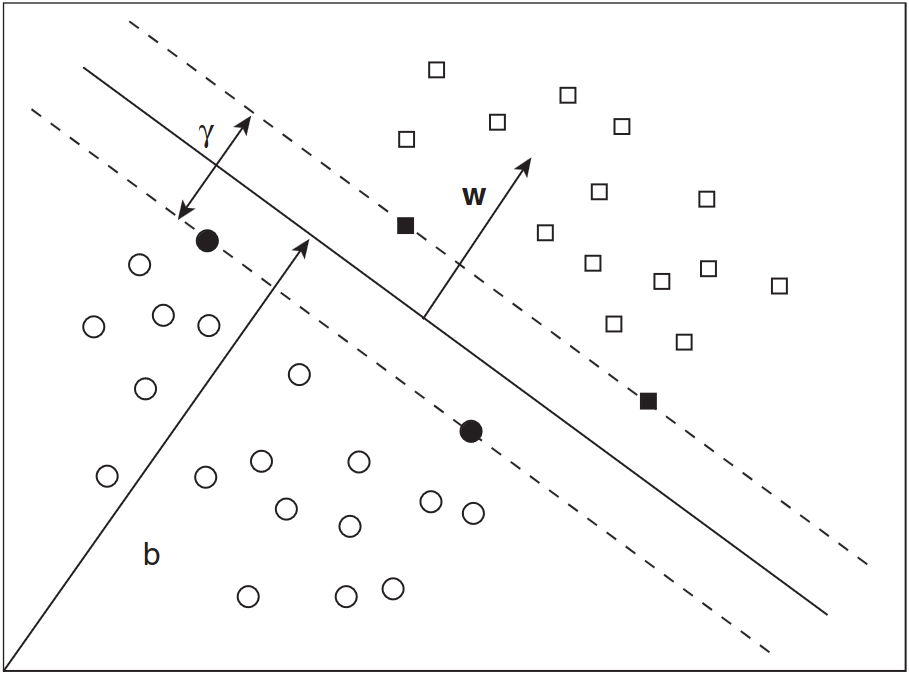
\includegraphics[width=0.5\linewidth]{images/svm.png}
    \caption{from ``Support vector machines" by Mammone\cite{mammone_support_2009}, A graphical rendering that outlines the steps taken in SVM linear classification in a two-dimensional feature space. In this model, circles and squares depict data points from two separate classifications. The solid line represents the hyperplane that was identified as the decision boundary by the SVM algorithm. Dotted lines are margins, and filled shapes (circles and squares) act as support vectors. Vector \textbf{w} is perpendicular to the hyperplane with a positive direction, while parameter \textbf{b} indicates how far off the origin the hyperplane lies. \textbf{y} is distance across each margin, which gets maxed out in SVM.}
    \label{fig:enter-label}
\end{figure}

Kernels are functions used in SVMs to transform your input data into a higher-dimensional space where it can then be separated more clearly with a hyperplane. This is particularly useful when you have non-linear separable problems. By mapping your low-dimensional feature space onto high-dimensional space, you're able to perform linear separation of data that is non-linearly separable in its original input space. \cite{mammone_support_2009}

When it comes to sound classification, SVMs could be used for differentiating between different types of sounds or determining characteristics of a single sound source. Support Vector Machines, in conjunction with a variety of feature extraction techniques, were utilized by the researchers to classify the types of stress experienced by plants, such as drought or physical damage like cuts. This involved basic features, Mel-frequency cepstral coefficients (MFCC), and a novel approach using scattering network. The SVM classifier was able to differentiate between different plant conditions (e.g., tomato or tobacco) and treatments (drought stress or cutting), thus enabling classification of the sound into specific types of stress.\cite{Cell_Sounds_emitted_by_plants}

It has been shown by means of the SVM classifier that when it is combined with scattering network for feature extraction, it can distinguish sounds of drought-stressed plants from those of physically damaged plants at a level of about 70\% for different species (tomato and tobacco). The model performed better than random chance in classification here, thus proving its ability to effectively discriminate diverse stress stimuli through ultrasonic sound emissions. Very similar results were conducted by a CNN classifier given the same task.\cite{Cell_Sounds_emitted_by_plants}


\noindent % Prevents indentation for this line
\begin{figure}[H]
  \centering
  \begin{subfigure}[b]{0.45\textwidth} % Adjust the width as needed
    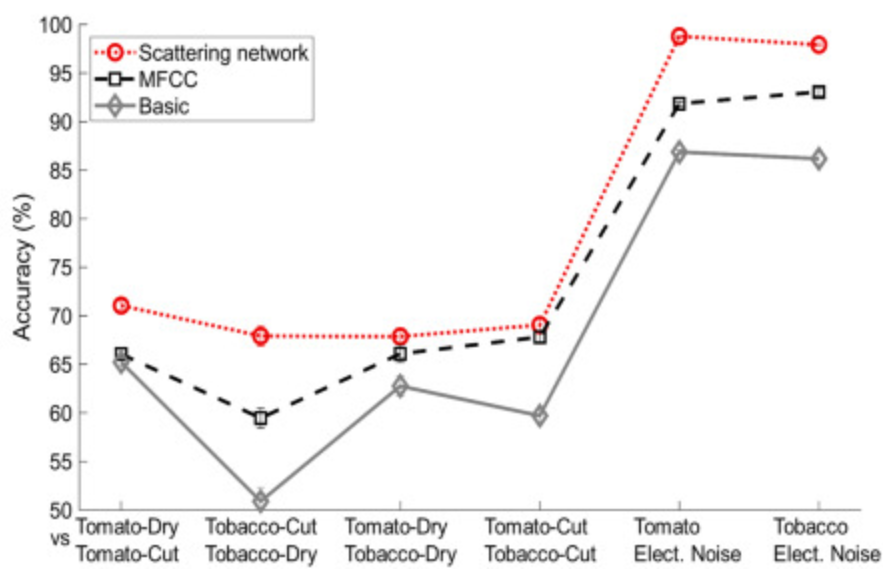
\includegraphics[width=\textwidth]{images/svm_classifier_results.png} % Adjust the image name and width as needed
    \caption{"The accuracy of sound classification achieved by different feature extraction methods, with an SVM classifier. The best results were obtained using the scattering network method for feature extraction (red). Using MFCC (black) for feature extraction the results were also highly significant and even basic methods (gray) for feature extraction allowed for better-than-random classification pair apart from one case: Tobacco dry vs. Tobacco cut, which was not significant with the basic method). The comparisons Tomato vs Elect. Noise and Tobacco vs Elect. Noise refer to electrical noise of the recording system." \cite{Cell_Sounds_emitted_by_plants}}
    \label{fig:image1}
  \end{subfigure}
  \hfill % Optional space between images
  \begin{subfigure}[b]{0.45\textwidth} % Adjust the width as needed
    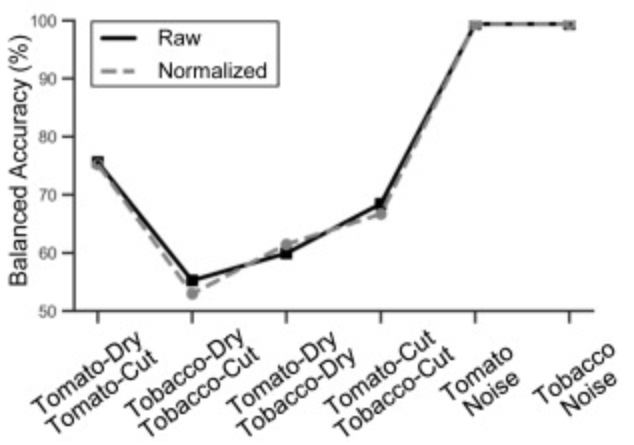
\includegraphics[width=\textwidth]{images/cnn_classifier_results.png} % Adjust the image name and width as needed
    \caption{"The accuracy of sound classification achieved by CNN models. The balanced accuracy of sound classification achieved by binary CNN models, for training and testing on the raw sound-vectors (black) and for training and testing on sound-vectors that were normalized by dividing each value in a vector by the vector’s maximal absolute value. Each balanced accuracy result is based on leave-one-plant-out cross validation." \cite{Cell_Sounds_emitted_by_plants}}
    \label{fig:image2}
  \end{subfigure}
  \caption{Comparison between SVM and CNN classifying plant stress type}
  \label{fig:images}
\end{figure}

\subsubsection{Leave-One-Plant-Out Cross-Validation (LOPO-CV)}
The Leave-One-Plant-Out Cross-Validation method was used to cross-validate the classification models. By treating every plant’s sound as a separate test set, this procedure makes the evaluation robust enough to withstand inter-plant variation bias within the samples. This approach serves more than one purpose: on the one hand it enhances generalizability; on the other hand, it provides direct proof that such models can work in real life situations involving variations from plant to plant.\cite{Cell_Sounds_emitted_by_plants}
